\subsection{Strahlensatz}

\hfill \break
Werden zwei von einem Punkt ausgehende Strahlen von zwei Parallellen Geschnitten, so lassen sich daraus bestimmte Verhältnisse abslesen. $\rightarrow$ Strahlensätze


\hfill \break
Regeln:
\begin{itemize}
    \item $a:b=c:d$
    \item $b*c=a*d$
\end{itemize}


\hfill \break
Beispiel für Strahlensätze:

\hfill \break
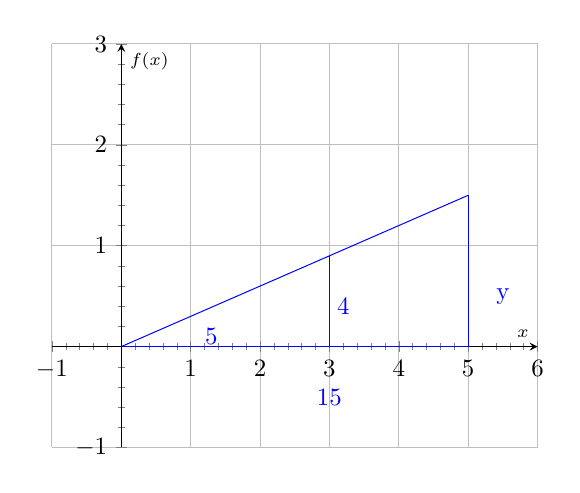
\begin{tikzpicture}[scale=0.9]
    \begin{axis}%
        [
            grid=major,
            xtick={-1,0,...,7},
            minor x tick num=4, % 4 minor ticks => 5 subintervals
            xmin=-1,
            xmax=6,
            xlabel={\scriptsize $x$},
            axis x line=middle,
            ytick={-1,0,...,3},
            minor y tick num=4,  % 4 minor ticks => 5 subintervals
            ymin=-1,
            ymax=3,
            ylabel={\scriptsize $f(x)$},
            axis y line=middle,
            no markers,
            samples=100,
            domain=-6:6,
        ]

        \draw[color=blue] (0,0) -- (5,1.5);
        \draw[color=blue] (5,0) -- (5,1.5);
        \draw[color=blue] (5,0) -- (0,0);
        \draw[color=blue] (3,0) -- (3,0.9);
        \node[color=blue] at (1.3,0.1) {5};
        \node[color=blue] at (3,-0.5) {15};
        \node[color=blue] at (5.5,0.5) {y};
        \node[color=blue] at (3.2,0.4) {4};
    \end{axis}
\end{tikzpicture}

\hfill \break
Example Verhältnisgleichung:\\
\fboxrule=0.8pt \fcolorbox{black}{lightgray}{%
    \begin{tabular}[t]{@{}l@{}}
        $5:4 = 15:y$ \\
        $5y = 60$    \\
        $y = 12$     \\
    \end{tabular}}
